\documentclass{article}
\usepackage{graphicx} % Required for inserting images
\usepackage[left=2cm,right=2cm,top=2cm,bottom=2cm]{geometry} 
\usepackage{setspace} 
\onehalfspacing
\usepackage{float}
\usepackage{fancyhdr}
\usepackage{booktabs}
\usepackage{array}
\usepackage{longtable}
\usepackage{geometry}
\usepackage{amsmath}
\usepackage{amsfonts}
\usepackage{mathrsfs}
\usepackage{hyperref}

\fancyhead[LO]{\small{\textit{Risk Theory: Assignment 2}}}

\title{\textbf{Risk Theory - Assignment 2}\\Econometrics and Data Science}
\author{
    Geesink, T. \\
    \texttt{14124165}
    }
    
\date{April 2026}

\begin{document}
    \pagestyle{fancy}

\includegraphics[scale=0.2]{logo.jpg}
\begingroup
{\let\newpage\relax\maketitle}
\maketitle
\endgroup 

\clearpage

\section*{Makeham and Gompertz mortality laws}

The purpose of this assignment is to review or learn about
\begin{itemize}
    \item mortality rates,
    \item Makeham and Gompertz mortality laws,
    \item determining maximum likelihood estimates for parameters,
    \item estimating expected lifetimes from the sample or from the cdfs using the maximum likelihood estimates of the parameters,
    \item proportional hazard models,
    \item the Akaike Information Criterion (AIC),
    \item making appropriate plots.
\end{itemize}

\section{Reading the data, basic calculations}

In the year 1899, 100\,000 people were born in the Netherlands. Their exact ages-at-death $X_i$ (in fractional years) were not recorded, but the integer parts $K_i = \lfloor X_i \rfloor$ were, for $i = 1, \ldots, 100\,000$. All their realized ages-at-death $k_1, \ldots, k_{100\,000}$ (integers) are known by now. They are summarized in a vector with the numbers of people $d_x$ that died at a particular age $x = 0, 1, \ldots, 94$. (The longest living person in this sample died at 94 years of age.) This vector of the `curtate lifetimes' can be read in R as follows:

\begin{verbatim}
d.x <- scan(text="
2618 390 85 41 26 26 30 32 34 33 22 37 28 32 25
20 36 38 29 27 30 38 28 38 52 33 48 49 45 48
51 55 56 55 67 76 82 104 92 114 94 121 139 152 163
205 196 237 275 296 343 382 421 526 582 622 742 878 921 1075
1216 1398 1594 1840 1923 2253 2483 2688 3186 3346 3710 3817 4121 4490 4688
4734 4864 4884 4756 4560 4120 3740 3385 2756 2079 1563 1086 727 455 228
103 42 17 7 1")
## numbers of people that died at ages x = 0,1,2,...,94
sum(d.x) ## returns 100000, as expected
\end{verbatim}

For our purposes, we do not need the full sample $k_1, k_2, \ldots, k_{100\,000}$ of the individual lifetimes; the numbers $d_x$ given above are sufficient.

Our first aim is to compute sample estimates of the probabilities of dying at age $x$ for our group of 1899-born people, given that they were alive on their $x$th birthday. We can do this by dividing the number $d_x$ of deaths at age $x$ by the number of people $n_x$ who were alive on their $x$th birthday. So we want to construct the vector $n_x$, using the values of $d_x$, for $x = 0, 1, \ldots, 94$. (Note that we ignore migration into and out of the population.)

The first entry in $n_x$ should be 100\,000, since all 100\,000 people in the sample were alive on their 0th birthday (i.e.\ moment of birth). The second entry in $n_x$ should be $100\,000 - 2\,618 = 97\,382$, since 2\,618 people died before reaching their first birthday. The third entry should be $97\,382 - 390 = 96\,992$, and so on, all the way to the 95th entry, which should be 1, because there was only one person who made it to his/her 94th birthday. (Simpler example: if we had $d_x = (1, 2, 3, 4, 5)$, then we would have $n_x = (15, 14, 12, 9, 5)$.)
\begin{enumerate}
\item[$\boldsymbol{Q_1}$] Construct the vector \texttt{n.x} of length 95, using the information in the vector \texttt{d.x}. Run \texttt{head(n.x, 3)} and \texttt{tail(n.x, 3)} to display the first and last 3 entries in \texttt{n.x}. Are they correct? (Hint: the R-functions \texttt{rev()} for reversing vectors and \texttt{cumsum()} for computing cumulative sums of vector entries might be useful.)
Now we can estimate the probabilities of dying at each age $x$, conditional on surviving up to the $x$th birthday, by computing the fractions $d_x/n_x$:
\begin{verbatim}
fr <- d.x/n.x
\end{verbatim}
A:
\begin{verbatim}
Output:
> n.x <- rev(cumsum(rev(d.x)))
> head(n.x, 3)
[1] 100000  97382  96992
> tail(n.x, 3)
[1] 25  8  1
\end{verbatim}
\newpage
\section{Makeham's mortality law}

Just by looking at the numbers in \texttt{d.x}, the observations $d_0, d_1, d_2$ can be seen to follow a different pattern than the remaining data. About 3\% of the newborns died while still infants. For the remaining 97\%, the ages-at-death are assumed to have arisen from a continuous lifetime distribution called Makeham's law or the Makeham distribution; see also exercise 3.9.16 in MART.

The mortality rate of a continuous random variable $X$ denoting a lifetime is defined as
\begin{equation}
\mu_X(x) \stackrel{\text{def}}{=} \frac{f_X(x)}{1 - F_X(x)}, \quad x > 0,
\end{equation}
where $f_X$ denotes the pdf (density) and $F_X$ denotes the cdf of $X$, as usual. By the chain rule, equation (1) is equivalent to
\begin{equation}
\mu_X(x) = -\frac{d}{dx} \log(1 - F_X(x)), \quad x > 0.
\end{equation}

We say that the lifetime $X$ has a $\text{Makeham}(a, b, c)$ distribution if $\mu_X(x) = a + bc^x$ for parameters $a \geq 0$, $b \geq 0$ and $c > 1$. Gompertz' law is the special case with $a = 0$.

Some remarks on mortality rates:
\begin{itemize}
    \item The mortality rate, aka the failure rate, characterizes a lifetime distribution just like the density or the cdf or the moment generating function.
    \item $f_X(x)\, dx$ can be interpreted as a newborn's probability of dying in the short time interval between $x$ and $x + dx$. Similarly, $\mu_X(x)\, dx = \frac{f_X(x)}{1-F_X(x)}\, dx$ can be interpreted as someone's conditional probability of dying in the short time interval between $x$ and $x + dx$, given that s/he is still alive at age $x$.
    \item If $X = \min\{Y, Z\}$ and $Y, Z$ are independent, then $\mu_X(x) = \mu_Y(x) + \mu_Z(x)$.
    \item By the last property, Makeham's mortality law $\mu_X(x) = a + bc^x$ can be seen as a competing risks model, since people die from whichever happens first:
    \begin{itemize}
        \item `accident' at age $Z \sim \text{Exponential}(a)$, with constant mortality rate $\mu_Z(x) = a$, or
        \item `death from old age' at age $Y \sim \text{Gompertz}(b, c)$, with exponentially increasing mortality rate $\mu_Y(x) = bc^x$.
    \end{itemize}
\end{itemize}

The mortality rate can be found from the cdf via (2). The opposite is also true: by taking integrals and then exponentials on both sides of (2), we get the following identity for the survival function $S_X(x) = 1 - F_X(x)$ of $X$:
\begin{equation}
S_X(x) = \exp\left(-\int_0^x \mu_X(t)\, dt\right), \quad x > 0.
\end{equation}

Applying formula (3) to the Makeham mortality rate $\mu_X(x) = a + bc^x$, we obtain the following survival function for the Makeham distribution:
\begin{equation}
S_X(x) = \exp\left(-ax - \frac{b}{\log c}(c^x - 1)\right), \quad x > 0.
\end{equation}

A simple R function to compute the survival function (4) for the Makeham distribution, with parameters $a \geq 0$, $b \geq 0$, $c > 1$, can be defined as follows:
\begin{verbatim}
sMakeham <- function (x, a, b, c) {
  ifelse(x<0, 1, exp(-a*x-b/log(c)*(c^x-1)))
}
\end{verbatim}

\item[$\boldsymbol{Q_2}$] (a) Assuming Makeham distribution for the lifetimes $X$, we want to write an R-function \texttt{dMakeham} to compute the probability of having curtate lifetime $K = \lfloor X \rfloor = 0, 1, \ldots$ That is, we want to compute
\[
\Pr[K = k] = \Pr\bigl[X \in [k, k+1)\bigr] = \Pr[X \geq k] - \Pr[X \geq k+1],
\]
for integer values $k = 0, 1, \ldots$ When $k$ is not integer, i.e.\ $k > \lfloor k \rfloor$, the probability $\Pr[K = k]$ should be zero. Note that because $S$ and $F$ are continuous, $\Pr[X \geq k] = \Pr[X > k] = S(k)$. Now using \texttt{sMakeham} defined above, fill in the dots to get the discrete density \texttt{dMakeham}:

\begin{verbatim}
dMakeham <- function (k, a, b, c) {
  ifelse(k>floor(k), 0, (sMakeham(...)-...))
}
\end{verbatim}
A:
\begin{verbatim}
sMakeham <- function (x, a, b, c) {
  ifelse(x < 0, 1, exp(-a * x - b / log(c) * (c^x - 1)))
}

dMakeham <- function (k, a, b, c) {
  ifelse(k > floor(k), 0, (sMakeham(k, a, b, c) - sMakeham(k + 1, a, b, c)))
}
\end{verbatim}


(b) As a quick sanity check for your answer to (a), run:
\begin{verbatim}
plot(dMakeham(0:100, 1e-4, 5e-5, 1.1), xlab="Age", ylab="")
\end{verbatim}
This will plot the \texttt{dMakeham} function for the age range 0--100, with parameter values $a = 10^{-4}$, $b = 5 \times 10^{-5}$ and $c = 1.1$. These parameter values correspond to a typical lifetime distribution in a developed country, so you should see a density that is mostly concentrated between the ages 40 and 100, with a peak around 80.
\newline \newline A:

\begin{figure}[H]
\centering
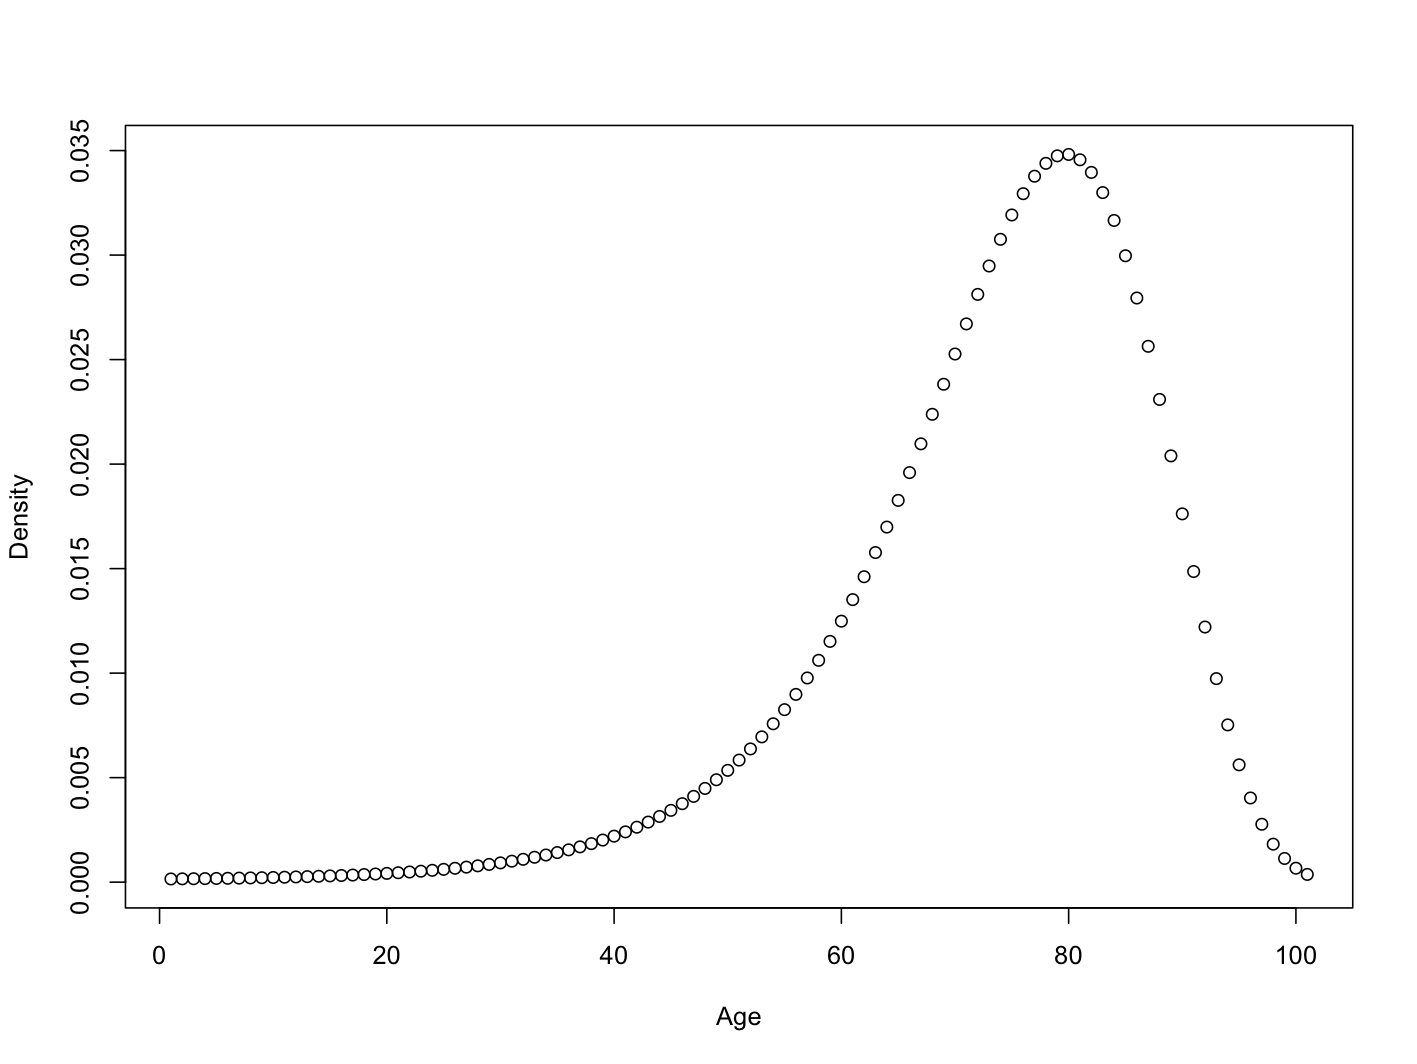
\includegraphics[width=0.6\textwidth]{Q2b.png}
\caption{Makeham density distribution with parameters $a = 10^{-4}$, $b = 5 \times 10^{-5}$, $c = 1.1$}
\end{figure}

\newpage
\subsection*{Graphically illustrating the data}
First we make a plot, of histogram type, of the table of lifetimes given in \texttt{d.x}. Note that rounded-down ages-at-death start at 0, but indices of vectors in R start at 1:
\begin{verbatim}
allages <- 0:(length(d.x)-1) ## ages from 0 to 94
plot(allages, d.x[allages+1], type="h")
\end{verbatim}

As we have noticed before, the first few counts stand out because of infant mortality. It looks like the lifetimes arise from a mixed distribution, with early deaths mostly caused by infant mortality, later ones following a Makeham distribution. To get estimates for the $a, b, c$ parameters of the Makeham distribution, one might replace the first few data points by fake ones following the pattern of the others. A better way is to simply ignore $d_0, d_1, d_2$ for the parameter estimation, considering only a subset of the ages $x$.
\begin{verbatim}
ages <- allages[allages>=3] ## ages from 3 to 94
plot(ages, d.x[ages+1], type="h")
\end{verbatim}
Now the plot looks very smooth, and similar to a Makeham density.

\section{Maximum likelihood estimates of the Makeham parameters}

The likelihood of the Makeham parameters $a, b, c$ is the probability under these parameters of our random sample $K_1 = k_1, K_2 = k_2, \ldots, K_{100\,000} = k_{100\,000}$, with $K_i = \lfloor X_i \rfloor$, therefore
\begin{equation}
L(a, b, c; k_1, \ldots, k_{100\,000}) = \prod_{i=1}^{100\,000} \Pr[K_i = k_i; a, b, c].
\end{equation}

By gathering terms with equal $k_i$ together, we can rewrite (5) as
\[
L(a, b, c; k_1, \ldots, k_{100\,000}) = \prod_{x=0}^{94} \bigl(\Pr[K = x; a, b, c]\bigr)^{d_x},
\]
since each age $x$ appears $d_x$ times in the product on the right-hand side of (5). Taking logarithms on both sides of the last equality, we get the following expression for the log-likelihood:
\[
\log L(a, b, c; k_1, \ldots, k_{100\,000}) = \sum_{x=0}^{94} d_x \log\bigl(\Pr[K = x; a, b, c]\bigr).
\]

Our aim is to find parameters $a, b, c$ that maximize this log-likelihood, using the \texttt{optim()} routine. The R-function \texttt{negloglikMakeham} below computes the negative log-likelihood. We compute the negative of the log-likelihood because maximizing the log-likelihood is equivalent to minimizing the negative log-likelihood, and \texttt{optim()} minimizes functions by default.

\begin{verbatim}
negloglikMakeham <- function (abc) {
  -sum(d.x[ages+1] * log(dMakeham(ages, abc[1], abc[2], abc[3])))
}
\end{verbatim}

In this function, \texttt{abc} is a vector of length 3 with values for $a, b, c$. Using \texttt{ages} rather than \texttt{allages}, we disregard sample elements with $k_i < 3$, which are dominated by infant mortality rather than influenced by the Makeham parameters.

\item[$\boldsymbol{Q_3}$] Minimize the function \texttt{negloglikMakeham} using the \texttt{optim()} routine. Use starting values \texttt{c(1e-4, 5e-5, 1.1)}, the parameter values we used in Q2(b) above. Store the optimization result in an object called \texttt{ooMakeham} and save the optimal parameter values as \texttt{a.hat}, \texttt{b.hat} and \texttt{c.hat}. These are the maximum likelihood estimates.

(Strictly speaking, we should make sure that we only search the feasible parameter space $a \geq 0$, $b \geq 0$ and $c > 1$, but since we have good starting values in this case, we can ignore this issue. You will see warnings produced by the \texttt{optim()} routine trying inadmissible parameter values during the search; you can ignore those warnings too.)
\newline \newline A:
\begin{verbatim}
negloglikMakeham <- function (abc) {
  # abc[1]=a, abc[2]=b, abc[3]=c
  -sum(d.x[ages+1] * log(dMakeham(ages, abc[1], abc[2], abc[3])))
}

ooMakeham <- optim(par = c(1e-4, 5e-5, 1.1), fn = negloglikMakeham)

a.hat <- ooMakeham$par[1]
b.hat <- ooMakeham$par[2]
c.hat <- ooMakeham$par[3]

Ouput:
> a.hat
[1] 0.0002767937
> b.hat
[1] 2.954879e-06
> c.hat
[1] 1.150241
\end{verbatim}
\newpage
\subsection*{Plotting estimated mortality rate and density}

Recall that in the vector \texttt{fr} (defined after Q1), we have saved the fractions of deaths at each age, conditional on survival up to that age. So \texttt{fr} is an estimate for the mortality rate at each age, directly obtained from data, without assuming any distribution for the lifetimes; we can call it a non-parametric estimate. An alternative, parametric estimate for the mortality rate is provided by the assumption of Makeham distribution on the data, namely: $\hat{\mu}(x) = \hat{a} + \hat{b}\, \hat{c}^x$. This is simply the Makeham mortality rate, with maximum likelihood estimates $\hat{a}, \hat{b}, \hat{c}$ plugged in for $a, b, c$. If the Makeham distribution is a good model for our dataset, these two mortality estimates (the non-parametric estimate \texttt{fr} and the Makeham estimate) should be close to each other. We can check this visually, by running:

\begin{verbatim}
plot(allages, fr, type="l") ## non-parametric mortality estimate
lines(allages, a.hat+b.hat*c.hat^allages, col="red") ## Makeham mort. est.
\end{verbatim}

Except at the very low and the very high ages, the two estimates are indeed pretty close to each other. At the very low ages, the difference is caused by infant mortality: the non-parametric estimate takes it into account, the Makeham estimate doesn't. At the very high ages, the non-parametric estimate becomes unreliable (and its graph becomes unstable), since there are too few survivors at those ages to yield reliable probability estimates.

We can also compare the estimated Makeham density with the observed fractions of people dying at ages $0, 1, \ldots, 94$, by running:

\begin{verbatim}
y <- d.x/sum(d.x) ## observed fractions of deaths at each age
plot(allages, y, type="h") ## plot observed fractions of deaths at each age
lines(allages, dMakeham(allages,a.hat,b.hat,c.hat), col="red") ## Makeham dens.
\end{verbatim}

After infant mortality, Makeham density fits the data rather well.

\section{Expected lifetime, number of retirement years}

For a person having lifetime $X \sim \text{Makeham}(a, b, c)$, the expected lifetime (or age-at-death) can be computed as
\[
\mathbb{E}[X] = \int_0^\infty S_X(x; a, b, c)\, dx,
\]
by MART (1.33) (with $d = 0$). This expected value can easily be estimated using the \texttt{integrate} function in R and filling in the estimates $\hat{a}, \hat{b}, \hat{c}$ for the parameters $a, b, c$:

\begin{verbatim}
integrate(sMakeham, 0, Inf, a.hat, b.hat, c.hat) ## 72.05
\end{verbatim}

To compute the sample average of the ages-at-death observed in our sample, we need to sum up all the ages-at-death and divide the result by the number of people in the sample (100\,000). We do this as follows:

\begin{verbatim}
sum((allages+0.5)*d.x) / sum(d.x) ## 69.86
\end{verbatim}
\newpage
\item[$\boldsymbol{Q_4}$] (a) Why is it reasonable to use \texttt{allages+0.5} rather than \texttt{allages} in the last computation?
\newline \newline A: The ages-at-death in the sample are given as integers, which represent the number of full years lived. 
For example, if someone died at age 65, it means they lived through their 65th birthday but did not reach their 66th birthday. 
Therefore, the actual age-at-death for someone recorded as dying at age $x$ is somewhere between $x$ and $x+1$. 
By adding 0.5 to each integer age, we are effectively estimating the average age-at-death for those who died at that age, assuming a uniform distribution of deaths within each year. 
This provides a more accurate estimate of the expected age-at-death than simply using the integer values.

(b) The expected age-at-death estimated via the sample average (69.86) is somewhat lower than the expected age-at-death estimated via the fitted Makeham distribution (72.05). Can you guess why that is the case?
\newline \newline A: 


\newpage
Next, we turn to the problem of estimating the expected number of pension years after age 65 for people born in 1899. For example, the \texttt{d.x[66]} = 2\,253 people who died at age 65 (that is, somewhere between their 65th and 66th birthdays) had on average one half pension year. Similarly, the \texttt{d.x[67]} = 2\,483 people who died at age 66 enjoyed an average of 1.5 pension years, etc. Anybody who died before reaching the age of 65 had zero pension years. So we can make a vector counting the number of pension years for each age-at-death, and compute the sample mean of pension years as follows:

\begin{verbatim}
pension.years <- pmax(allages + 0.5 - 65, 0)
sum(pension.years*d.x) / sum(d.x) ## 8.62
\end{verbatim}

So the people in our sample have spent an average of 8.62 years in retirement.

\item[$\boldsymbol{Q_5}$] Now estimate the expected number of pension years $\mathbb{E}[(X - 65)^+]$ for a person with age-at-death $X \sim \text{Makeham}(\hat{a}, \hat{b}, \hat{c})$. (Hint: use MART (1.33) and \texttt{integrate()}.) This estimate should be somewhat higher than the sample estimate 8.62 computed above. Can you explain why?
\newline \newline A:
\begin{verbatim}
exp_pension <- integrate(sMakeham, 65, Inf, a.hat, b.hat, c.hat)$value
output:
> exp_pension
[1] 8.898422
\end{verbatim}


\newpage
\item[$\boldsymbol{Q_6}$] (a) Another quantity of interest is the average number of pension years only for those people who have actually reached the pension age 65. Compute this quantity from the sample, by restricting the sample average computation above to ages with \texttt{pension.years} positive. (Hint: the result should be higher than 8.62, since we are disregarding all the people who have spent zero years in retirement.)
\newline \newline A:
\begin{verbatim}
pension.years <- pmax(allages + 0.5 - 65, 0)
sample_cond <- sum(pension.years * d.x) / sum(d.x[allages >= 65])

output:
> sample_cond
[1] 10.93205
\end{verbatim}

(b) Now estimate the expected number of pension years $\mathbb{E}[X - 65 \mid X > 65]$ for a person with age-at-death $X \sim \text{Makeham}(\hat{a}, \hat{b}, \hat{c})$, conditional on this person reaching the age of 65. (Hint: since this person is known to exceed the age of 65, his/her survival function is $S_X(x)/S_X(65)$, for $x > 65$. We have seen before Q4 how to compute the expected value from the survival function.)
\newline \newline A:
\begin{verbatim}
makeham_cond <- integrate(sMakeham, 65, Inf, a.hat, b.hat, c.hat)$value / sMakeham(65, a.hat, b.hat, c.hat)

Output:
> makeham_cond
[1] 10.94129
\end{verbatim}

(c) You should see that the Makeham estimate in part (b) of the expected number of pension years for people surviving up to age 65 is quite close to the corresponding sample estimate in (a), even though the Makeham estimate in Q5 of the expected number of pension years for everybody was higher than the corresponding sample estimate. Can you explain why this is the case?
\newline \newline A:



\newpage
\section{Proportional hazard models}

It is sometimes claimed that because of smoking, mortality rates are multiplied by a certain factor, let's say, doubled. We want to investigate what effect doubling the mortality rate has on the life expectancy.

\item[$\boldsymbol{Q_7}$] Let $X$ be a random variable denoting the lifetime (or age-at-death) of a person, with corresponding mortality rate $\mu_X(x)$ and survival function $S_X(x)$. Note that we are not assuming $X$ to be Makeham. Suppose the mortality rate $\mu_X$ gets multiplied by a factor $f$ (perhaps due to smoking) to yield a new mortality rate $\mu_X^{\text{new}}(x) = f \cdot \mu_X(x)$. Use equation (3) to express the new survival function $S_X^{\text{new}}(x)$ in terms of the original survival function $S_X(x)$.
\newline \newline A:


\newpage
\item[$\boldsymbol{Q_8}$] Now imagine a person having lifetime $X \sim \text{Makeham}(\hat{a}, \hat{b}, \hat{c})$, with $\hat{a}, \hat{b}, \hat{c}$ as computed in Q3.

(a) Using the \texttt{integrate} function as before (beginning of Section 4), compute the expected age-at-death for this person, if the mortality rate gets multiplied by a factor $f = 2^k$, $k = -3, -2, -1, 0, 1, 2, 3$. Store the resulting (seven) expected ages-at-death in a vector called \texttt{exp.lifetimes}. (Hint: you can use the result of Q7, or the fact that multiplying the Makeham mortality rate $\hat{a} + \hat{b}\, \hat{c}^x$ by $f$ means replacing $\hat{a}$ with $f \cdot \hat{a}$ and $\hat{b}$ with $f \cdot \hat{b}$.)
\newline \newline A:
\begin{verbatim}
k_vals <- -3:3
f_vals <- 2^k_vals
exp.lifetimes <- sapply(f_vals, function(f) {
  integrate(function(x) sMakeham(x, a.hat, b.hat, c.hat)^f, 0, Inf)$value
})
\end{verbatim}

(b) Plot the \texttt{exp.lifetimes} against $k$, and conclude that the expected age-at-death drops roughly by the same amount (number of years) every time the mortality rate gets doubled (i.e.\ $k$ increases by 1). What is that amount?
\newline \newline A:
\begin{figure}[H]
\centering
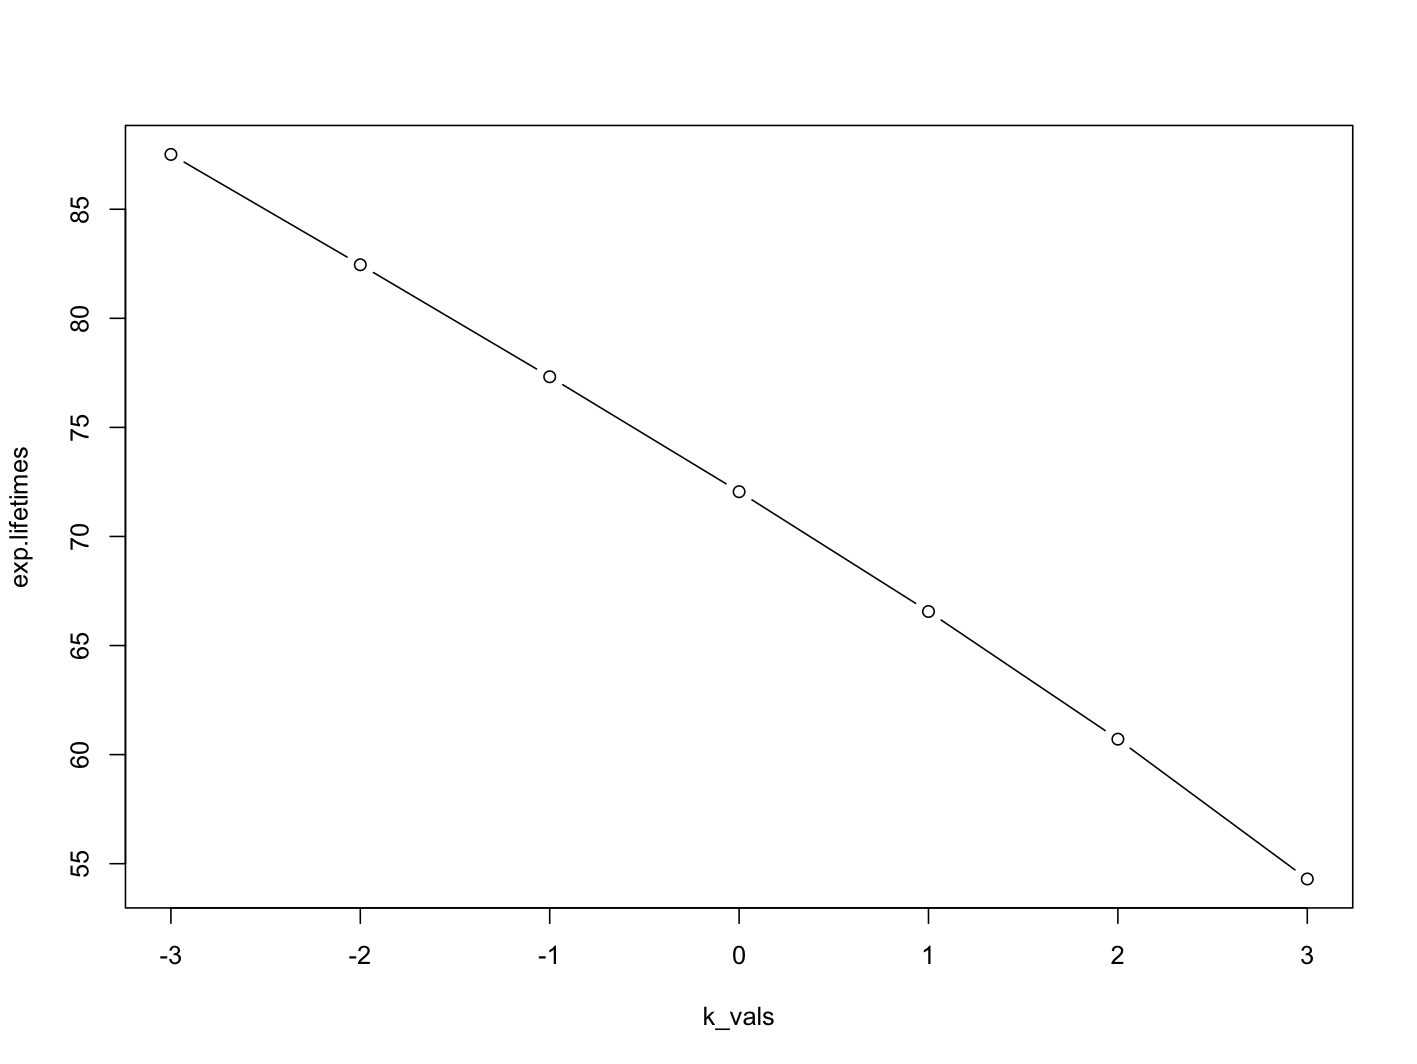
\includegraphics[width=0.6\textwidth]{Q8b.png}
\caption{Expected age-at-death as a function of $k$, where $f = 2^k$ is the factor by which the mortality rate is multiplied.}
\end{figure}

\newpage
\section{Reducing Makeham's law to Gompertz'}

As mentioned before, Gompertz' law is the same as Makeham's law, but with $a = 0$. Recall that we interpreted Makeham's mortality rate $a + bc^x$ as a ``competing risks'' model, where constant mortality $a$ is contributed by a constant (low) risk of dying from an ``accident'' at any moment, and mortality $bc^x$ is contributed by an exponentially increasing risk of dying from ``old age''. From this point of view, the Gompertz model ignores the ``accident'' component and assumes that people only die from ``old age''.

\item[$\boldsymbol{Q_9}$] (a) Repeat the steps in Section 3 to compute maximum likelihood estimates $\hat{b}$ and $\hat{c}$ for the Gompertz parameters $b$ and $c$, using the data in \texttt{d.x}. Store the parameter estimates as \texttt{b.hat.Gompertz} and \texttt{c.hat.Gompertz}. (Hint: as starting values for the optimization, you can use the Makeham estimates \texttt{b.hat} and \texttt{c.hat}.)
\newline \newline A:
\begin{verbatim}
negloglikGompertz <- function (bc) {
  -sum(d.x[ages+1] * log(dMakeham(ages, 0, bc[1], bc[2])))
}
ooGompertz <- optim(par = c(b.hat, c.hat), fn = negloglikGompertz)

b.hat.Gompertz <- ooGompertz$par[1]
c.hat.Gompertz <- ooGompertz$par[2]

Output:
> b.hat.Gompertz
[1] 5.374668e-06
> c.hat.Gompertz
[1] 1.141095
\end{verbatim}
\newpage
(b) As in Section 3, plot the observed fractions $d_x/100\,000$ of people dying at each age $x$, together with the fitted Makeham density and the fitted Gompertz density. (Produce a single plot, use different colors for the two densities.) Can you tell from the plot which distribution fits the data better?
\newline \newline A:
\begin{verbatim}
dGompertz <- function(k, b, c) {
  dMakeham(k, 0, b, c)
}

a_m <- ooMakeham$par[1]
b_m <- ooMakeham$par[2]
c_m <- ooMakeham$par[3]

b_g <- ooGompertz$par[1]
c_g <- ooGompertz$par[2]

ages_plot <- 0:94
obs_fractions <- d.x / 100000

plot(ages_plot, obs_fractions, type = "p", pch = 16, cex = 0.6,
     xlab = "Age (x)", ylab = "Density / Fraction of Deaths",
     main = "Observed vs. Fitted Mortality Densities")

lines(ages_plot, dMakeham(ages_plot, a_m, b_m, c_m), col = "red", lwd = 2) # Makeham Density

lines(ages_plot, dGompertz(ages_plot, b_g, c_g), col = "blue", lwd = 2, lty = 2) # Gompertz Density

legend("topleft", legend = c("Observed (dx/100k)", "Makeham Fit", "Gompertz Fit"),
       col = c("black", "red", "blue"), pch = c(16, NA, NA), lty = c(NA, 1, 2), lwd = 2)
\end{verbatim}
\begin{figure}[H]
\centering
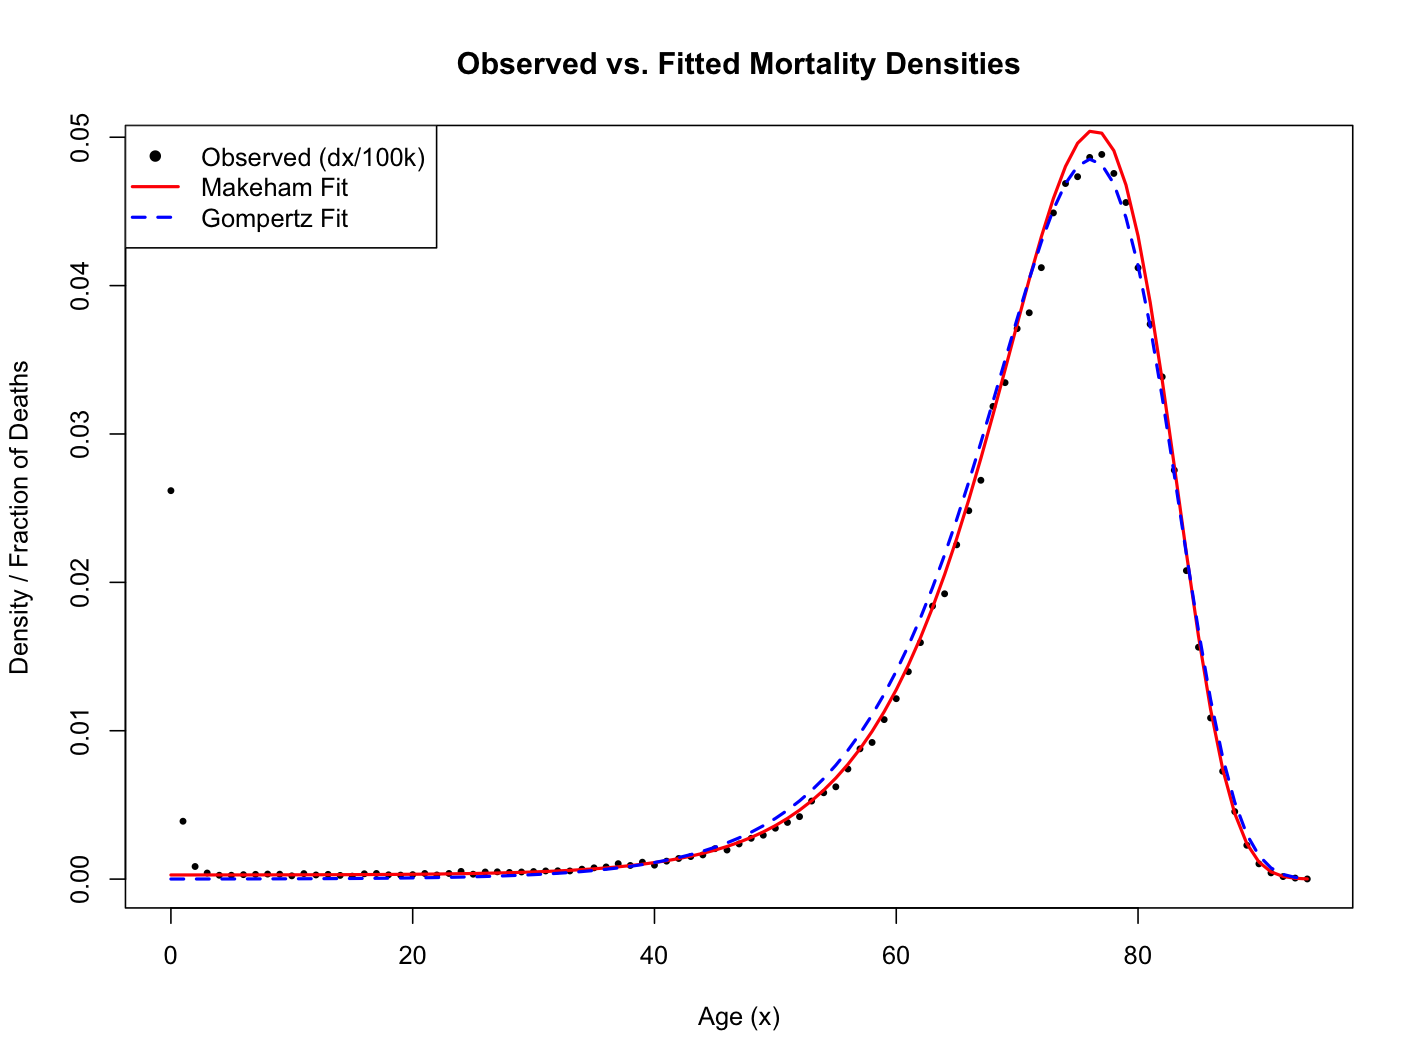
\includegraphics[width=0.6\textwidth]{Q9b.png}
\caption{Observed fractions of deaths at each age, together with fitted Makeham and Gompertz densities.}
\end{figure}

\newpage
(c) One possible way of comparing the fit of two parametric models for a given dataset is the Akaike Information Criterion, or AIC for short. The AIC for a parametric model is defined as $2k - 2\ell$, where $k$ is the number of parameters estimated in the model (3 for Makeham, 2 for Gompertz), and $\ell$ is the maximized value of the log-likelihood function for the estimated model. According to statistical theory, the model with the lower AIC value provides a better fit to the dataset. Note that this method ``rewards'' a high likelihood, but ``penalizes'' the use of too many parameters.
Compute the AIC values for both the Makeham and the Gompertz models. Which model fits better according to the AIC?
\newline \newline A:
\begin{verbatim}
aic_makeham <- 2*3 - 2*(-ooMakeham$value)
aic_gompertz <- 2*2 - 2*(-ooGompertz$value)

output:
> aic_makeham
[1] 699908.4
> aic_gompertz
[1] 702167.6
\end{verbatim}
The Makeham model has a lower AIC value (699908.4) compared to the Gompertz model (702167.6), indicating that the Makeham model provides a better fit to the dataset according to the AIC criterion.

\end{enumerate}
\end{document}
